% 
% در این بخش یک نمونه آورده می‌شود و گرافهای ترسیم شده توسط داگزی در آن نمایش داده
% می‌شود. این نمونه برا اساس مستندهای خود داگزی ایجاد شده است
% 
% \author maso
% \date تابستان ۱۳۹۱
% 
\section{یک نمونه ساده}

در این بخش با استفاده از یک نمونه، تصویر روشنی از نمودارهای ایجاد شده در مستند
ایجاد خواهد شد. نمونه مورد استفاده در این بخش تنها به منظور نمایش قابلیت‌های این
ابزار در به کارگیری نمودارها ایجاد شده است از این رو بسیار ساده در نظر گرفته شده
است. در عین حال تلاش شده است که نمونه به گونه‌ای ایجاد شود که بتواند جنبه‌های
متفاوتی از گراف و نمودارها را به نمایش بگذارد.


در این نمونه از زبان برنامه سازی \lr{C/C++} استفاده شده است، که می‌تواند با
زبانهای برنامه سازی دیگر مانند \lr{Java}، \lr{PHP} و غیره جایگزین شود. در گام
نخست یک پرونده سرآیند به نام \lr{diagram\_a.h} ایجاد کرده و متن زیر را
\glspl{computer::copy} و در آن \glspl{computer::paste} کنید.

\begin{C++}
/**
 * \file diagram_a.h
 *
 * \author Arsheet.org
 * \date Summer 1391
 */
#ifndef DIAGRAM_A_H_
#define DIAGRAM_A_H_
class A {
public:
	A *m_parent;
};
#endif /* DIAGRAM_A_H_ */
\end{C++}

این قطعه کد معادل با ایجاد یک موجودیت به نام \lr{A} است که یک رابطه با خودش
دارد. رابطه موجود در این موجودیت به نام \lr{m\_parent} تعریف و در
عمل به عنوان موجودیت پدر آن در نظر گرفته شده است. در حالت عادی دو نوع نمودار
برای این موجودیت ایجاد خواهد شد که در شکل \ref{image/write/graph/example/class-a}
نمایش داده شده است. این نمودارها به ترتیب نمودار \glspl{collaboration diagram} و
\glspl{inheritance diagram} است.

% FIXME: maso 1391: این نمایش از تصاویر مناسب نیست و باید به صورت کامل اصلاح شود
\begin{figure}
    \centering
    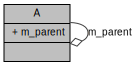
\includegraphics[width=0.4\textwidth]{write/graph/example/class_a__coll__graph}
    \label{image/write/graph/example/class_a__coll__graph}
\end{figure}

\begin{figure}
    \centering
    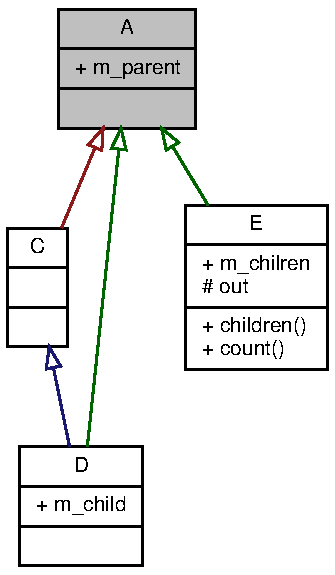
\includegraphics[width=0.4\textwidth]{write/graph/example/class_a__inherit__graph}
    \label{image/write/graph/example/class_a__inherit__graph}
\end{figure}

علاوه بر این نیز، در مستندها نمودارهایی نیز برای نمایش رابطه میان پرونده‌ها
ایجاد می‌شود. از جمله این نمودارها می‌توان به نمودار \glspl{include graph} و
\glspl{include by graph} اشاره کرد. نمودار \glspl{include by graph} برای این
نمونه نیز در شکل \ref{image/write/graph/example/diagram__a_8h__dep__incl} نمایش
داده شده است. با استفاده از این نوع نمودارها نه تنها پرونده‌های مورد استفاده در
یک پرونده و یا سرآیند خاص بلکه پرونده‌هایی که از پرونده مورد نظر نیز استفاده
کرده‌اند نمایش داده می‌شود. در هر نمودار تنها یک پرونده مورد نظر بوده و تمام
رابطه‌های نمایش داده شده بر اساس آن پرونده ایجاد خواهد شد. برای نمونه پرونده
مورد نظر در شکل \ref{image/write/graph/example/diagram__a_8h__dep__incl} پرونده
سرآیند \lr{diagram\_a.h} است که در نمودار با رنگه تیره‌تر نمایش داده شده است، از
این رو دیگر پرونده‌های نمایش داده شده پرونده‌هایی هستند که به صورت مستقیم و یا
غیر مستقیم از این پرنده استفاده کرده‌اند.

% FIXME: maso 1391: این نمایش از تصاویر مناسب نیست و باید به صورت کامل اصلاح شود
\begin{figure}
	\centering
	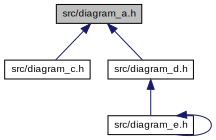
\includegraphics[width=0.5\textwidth]{image/write/graph/example/diagram__a_8h__dep__incl}
	\caption[نمونه]{
		نمونه
	}
	\label{image/write/graph/example/diagram__a_8h__dep__incl}
\end{figure}

\begin{note}
در شکلهای \ref{image/write/graph/example/class-a} و
\ref{image/write/graph/example/diagram__a_8h__dep__incl}
موجودیت، پرونده و یا کالس‌هایی نمایش داده شده‌اند که پیش از این نامی از آنها
برده نشده است. این موجودیت‌ها در ادامه به صورت مجزا تعرف شده و مورد بحث قرار
خواهند گرفت. از آنجا که این نمودارها بر اساس نمونه کامل ایجاد شده است، تمام
موجودیت‌های تعریف شده در نمونه در آن آورده شده است.
\end{note}

در عمل سیستم‌های طراحی شده بسیار پیچیده‌تر از این نمونه‌ای است که در اینجا آورده
شده است. برای نمونه در ساده ترین سیستم ها وراثت میان موجودیت‌ها استفاده شده است
در حالی که در موجودیت \lr{A} حتی از این مفاهیم ساده نیز به کاربرده نشده. با این
وجود \lr{Doxygen} رابطه‌های پیچیده میان موجودیت‌ها را تشخیص داده و نمودارهای
مناسب را برای آنها ایجاد می‌کند.

در ادامه یک پرنده سرآیند دیگر به نام \lr{diagram\_b.h} ایجاد کنید. موجودیتی به
نام \lr{B} ایجاد خواهد شد که یک وابستگی به موجودیت \lr{A} دارد. کد این پرنده را
به صورت زیر در نظر بگیرید.

\begin{C++}
/**
 * \file diagram_b.h
 *
 * \author Arsheet.org
 * \date Summer 1391
 */
#ifndef DIAGRAM_B_H_
#define DIAGRAM_B_H_
class A;
class B {
public:
	A *m_friend;
};
#endif /* DIAGRAM_B_H_ */
\end{C++}

در این قطعه کد یک موجودیت جدید به نام \lr{B} ایجاد شده است که یک رابطه با
موجودیت \lr{A} دارد. این رابطه در این کلاس به نام \lr{m\_friend} در نظر گرفته
شده است. با تولید مستند از این کلاس و ایجاد \glspl{collaboration diagram}
نموداری مشابه با شکل \ref{image/write/graph/example/class_b__coll__graph} ایجاد
خواهد شد. در این نمودار نه تنها نوع رابطه بلکه نام آن نیز نمایش داده می‌شود.

% FIXME: maso 1391: این نمایش از تصاویر مناسب نیست و باید به صورت کامل اصلاح شود
\begin{figure}
	\centering
	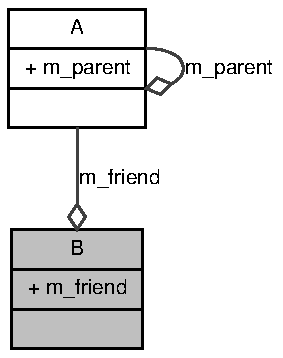
\includegraphics[width=0.5\textwidth]{image/write/graph/example/class_b__coll__graph}
	\caption[نمونه]{
		نمونه
	}
	\label{image/write/graph/example/class_b__coll__graph}
\end{figure}

با پیچیده‌تر شدن ساختار رابطه‌ای یک کلاس، ساختار رابطه‌ای میان پرونده‌ها و
سرایندها نیز پیچیده‌تر خواهد شد. در این حالت برای پیاده سازی یک کلاس ممکن است
نیاز به استفاده از سرایندهای متفاوتی باشد که گاها برخی از آنها در ساختار پروژه
نیز وجود ندارند.
برای نمونه پرونده سرآیند دیگری را به نام \lr{diagram\_c.h} در نظر بگیرید. در این
پرونده از سرایندهای متفاوتی استفاده شده است که برخی در ساختار پروژه و برخی از
کتابخانه‌های تعریف شده در خود سیستم است. کد این پرنده به صورت زیر است:

% پرنده‌ها
\begin{C++}
/**
 * \file diagram_c.h
 *
 * \author Arsheet.org
 * \date Summer 1391
 */
#include "diagram_a.h"
#include <math.h>
#include <iostream>
#include <stdlib.h>
#ifndef DIAGRAM_C_H_
#define DIAGRAM_C_H_
class A;
class C: private A {
public:
	A *m_left
}
#endif /* DIAGRAM_C_H_ */
\end{C++}

در این قطعه کد از چهار پرونده سرآیند استفاده شده است که اولین انها در ساختار
پروزه و مابقی بر اساس بسته‌های استاندارد زبان برنامه سازی \lr{C/C++} است.
\glspl{include graph} برای این پرونده در شکل
\ref{image/write/graph/example/diagram__c_8h__incl} نمایش داده شده است.

% FIXME: maso 1391: این نمایش از تصاویر مناسب نیست و باید به صورت کامل اصلاح شود
\begin{figure}
	\centering
	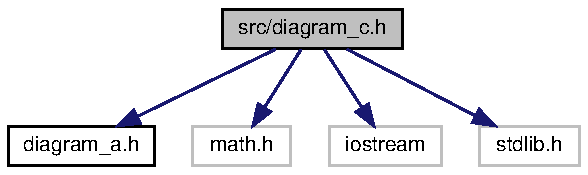
\includegraphics[width=0.5\textwidth]{image/write/graph/example/diagram__c_8h__incl}
	\caption[نمونه]{
		نمونه
	}
	\label{image/write/graph/example/diagram__c_8h__incl}
\end{figure}

در این نمودار تنها پروندهها و سرآیندهایی نمایش داده خواهند شد که در پرونده مورد
نظر مورد استفاده قرار گرفته‌اند و از سایر پرونده‌ها صرف نظر خواهد شد. از انجا که
همواره پرونده اصلی در این نمودار به عنوان مبنا قرار خواهد گرفت، این پرونده با یک
رنگ تیره‌تر نمایش داده خواهد شد.

گونه‌ای دیگر از رابطه‌ها که در زبان برنامه سازی \lr{C/C++} بسیار مرسوم است،
استفاده از وراثت‌های چندگانه است. برای نمونه کد زیر یک کلاس جدید به نام \lr{D}
ایجاد شده است که نه تنها شامل رابطه وراثت بلکه رابطه‌هایی پیچیده تر نسبت به
نمونه‌ها قبلی است.

\begin{C++}
/**
 * \file diagram_d.h
 *
 * \author Arsheet.org
 * \date Summer 1391
 */
#include "diagram_a.h"
#include "diagram_b.h"
#ifndef DIAGRAM_D_H_
#define DIAGRAM_D_H_
class C;
class A;
class B;
class D: virtual protected A, private B , public C{
public:
	C m_child;
};
#endif /* DIAGRAM_D_H_ */
\end{C++}

در این نمونه نه تنها کلاس ایجاد شده شامل چندین وراثت است بلکه، سطح دسترسی به هر
کدام متفاوت است. کلاس \lr{D} به صورت \glspl{public} از کلاس \lr{C} توسعه
یافته است در حالی که وراثت آن از کلاس \lr{B} به صورت \glspl{private} است. این
کلاس علاوه بر این دو نوع وراثت، یک وراثت دیگر از نوع \glspl{protected} از کلاس
\lr{A} دارد. \glspl{inheritance diagram} تولید شده از این کلاس در شکل
\ref{image/write/graph/example/class_d__inherit__graph} نمایش داده شده است.

% FIXME: maso 1391: این نمایش از تصاویر مناسب نیست و باید به صورت کامل اصلاح شود
\begin{figure}
	\centering
	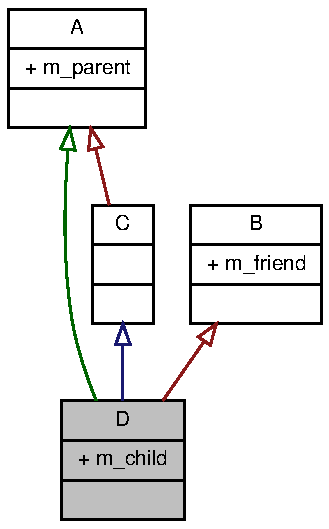
\includegraphics[width=0.5\textwidth]{image/write/graph/example/class_d__inherit__graph}
	\caption[نمونه]{
		نمونه
	}
	\label{image/write/graph/example/class_d__inherit__graph}
\end{figure}

با یک نگاه سطح در شکل \ref{image/write/graph/example/class_d__inherit__graph} به
این نکته پی خواهید برد که در این نمودار نوع هر رابطه را با استفاده از یک رنگ
نمایش داده شده است. برای نمونه وراثت از نوع \glspl{private} به رنگ قرمز و
\glspl{public} به رنگ مشکی نمایش داده شده است.

\lr{Doxygen} نه تنها \glspl{collaboration diagram} را مبتنی بر کلاس‌ها و
موجودیت‌های موجود در پروژه ایجاد کرده بلکه توانایی ایجاد رابطه‌های مناسب برای
نمونه‌هایی که خارج از پروژه ایجاد شده‌اند را نیز دارد. برای نمونه حالت زیر را در
نظر بگیرید که در آن از مجراهای ورودی استفاده شده است. این نمونه در یک پرونده
جدید به نام \lr{diagram\_e.h} پیاده سازی شده که کد آن به صورت زیر است:

% وراثت چند گانه
\begin{C++}
/**
 * \file diagram_e.h
 *
 * \author Arsheet.org
 * \date Summer 1391
 */
#include "diagram_d.h"
#include <vector>
#include <iostream>
#ifndef DIAGRAM_E_H_
#define DIAGRAM_E_H_
#include "diagram_e.h"
class C;
class A;
class B;
class E: virtual protected A, private B {
private:
	int m_count;
protected:
	iostream* out;
public:
	vector<C> m_chilren;
public:
	vector<C>* children();
	int count();
};
#endif /* DIAGRAM_E_H_ */
\end{C++}

\glspl{collaboration diagram} ایجاد شده از این کلاس در شکل
\ref{image/write/graph/example/class_e__coll__graph} نمایش داده شده است.


% FIXME: maso 1391: این نمایش از تصاویر مناسب نیست و باید به صورت کامل اصلاح شود
\begin{figure}
	\centering
	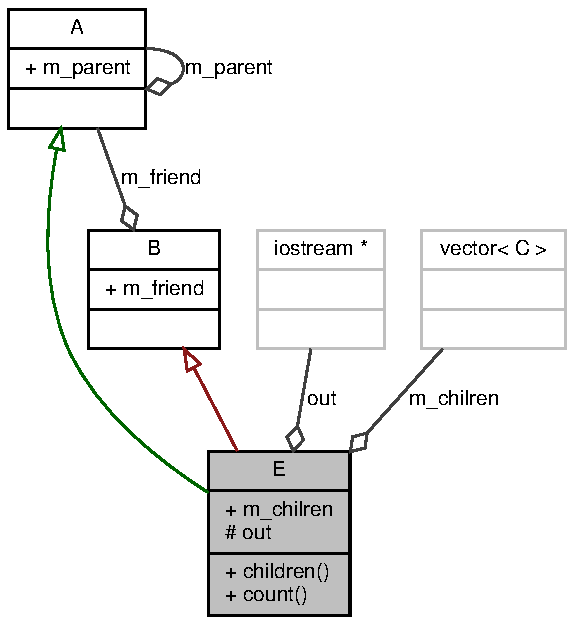
\includegraphics[width=0.5\textwidth]{image/write/graph/example/class_e__coll__graph}
	\caption[نمونه]{
		نمونه
	}
	\label{image/write/graph/example/class_e__coll__graph}
\end{figure}

% 
% FIXME: maso 1391: دانلود کد نمونه
% بهتر است که کد ایجاد شده برای این نمونه در یک مسیر روی اینترنت قرار گرفته شده
% باشد تا کاربران بتوانند ان را دانلود کرده و مورد استفاده قرار دهند.
% 
